\section{Similarity Measures}
\begin{frame}{}
    \LARGE Similarity Measures
\end{frame}

\begin{frame}{Vector Space}
    \begin{figure}
        \centering
        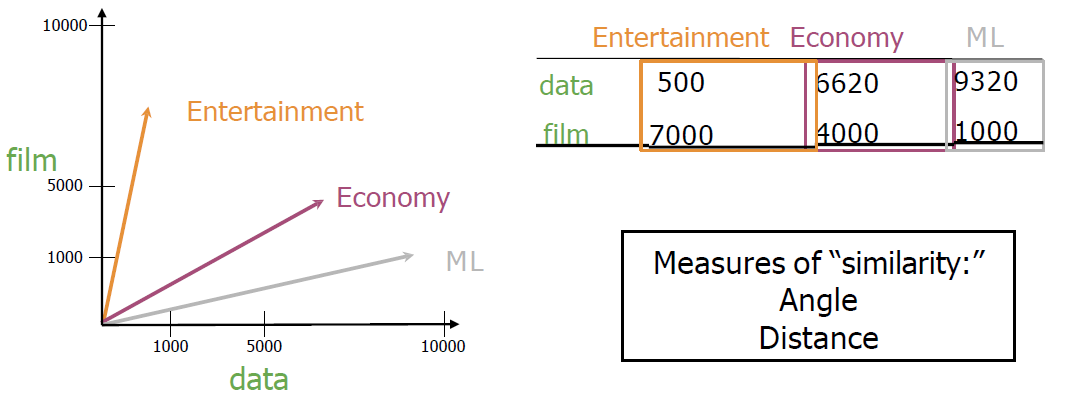
\includegraphics[width=\textwidth,height=0.8\textheight,keepaspectratio]{images/vector-space/vector-space.png}
    \end{figure}
\end{frame}

\subsection{Euclidean Distance}
\begin{frame}[allowframebreaks]{Euclidean Distance}
    \begin{figure}
        \centering
        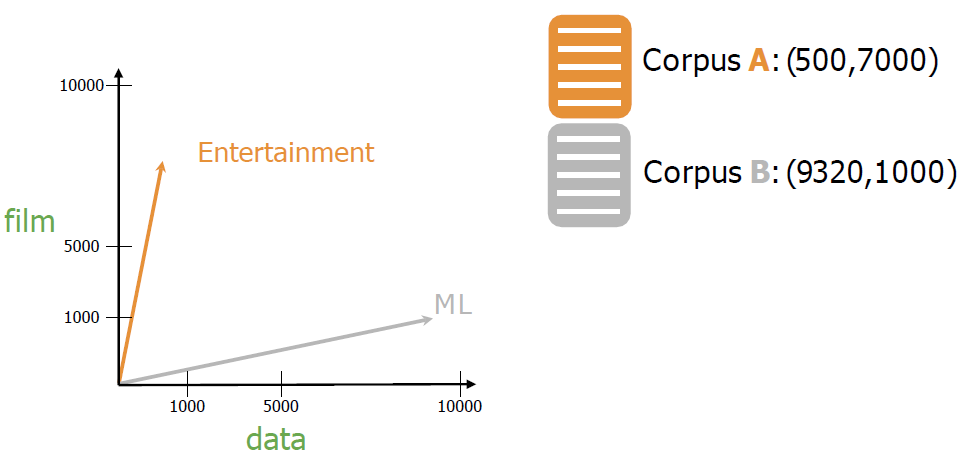
\includegraphics[width=\textwidth,height=0.65\textheight,keepaspectratio]{images/vector-space/euclidean-distance-1.png}
    \end{figure}
    \begin{itemize}
        \item Measures the straight-line distance between two points in space.
        \item Formula: $d(\mathbf{x}, \mathbf{y}) = \sqrt{\sum_{i=1}^{n} (x_i - y_i)^2}$
        \item Sensitive to the scale (magnitude) of the vectors.
    \end{itemize}
\framebreak
    \begin{figure}
        \centering
        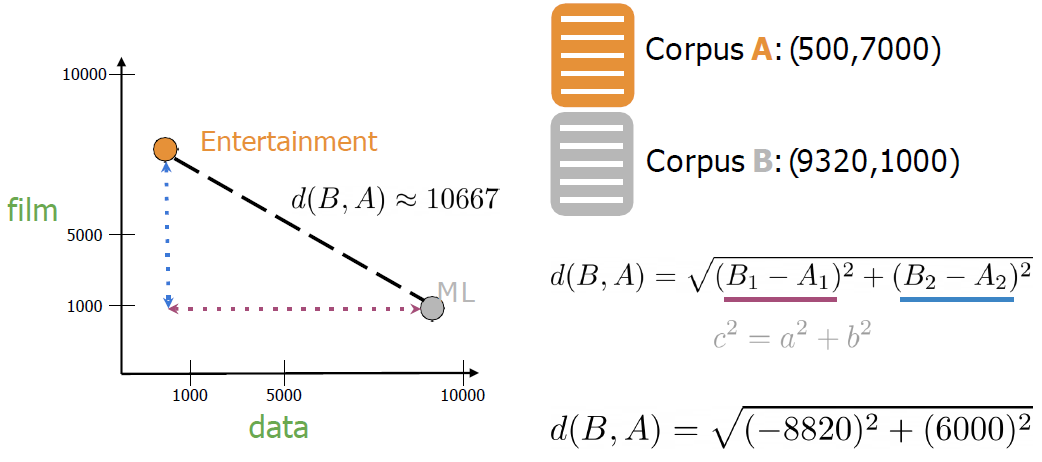
\includegraphics[width=\textwidth,height=0.65\textheight,keepaspectratio]{images/vector-space/euclidean-distance-2.png}
    \end{figure}
\end{frame}

\begin{frame}[allowframebreaks]{Euclidean Distance for n-dimensional vectors} 
    \begin{figure}
        \centering
        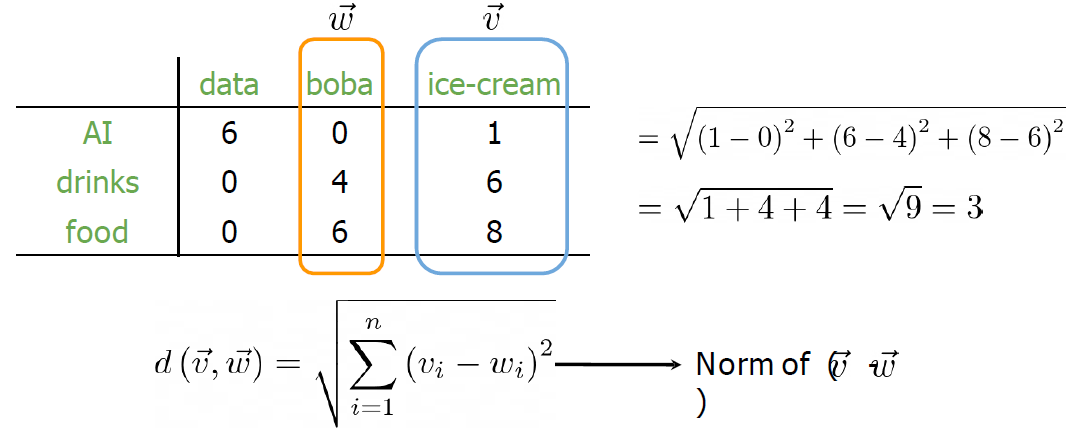
\includegraphics[width=\textwidth,height=0.65\textheight,keepaspectratio]{images/vector-space/euclidean-distance-3.png}
    \end{figure}
\end{frame}

\begin{frame}[allowframebreaks]{Euclidean Distance in Python} 
    \begin{figure}
        \centering
        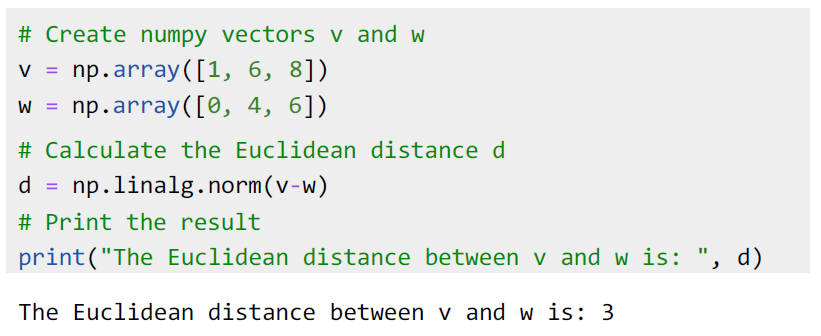
\includegraphics[width=\textwidth,height=0.65\textheight,keepaspectratio]{images/vector-space/euclidean-distance-4.png}
    \end{figure}
\end{frame}

\subsection{Cosine Similarity}
\begin{frame}[allowframebreaks]{Cosine Similarity}
    \begin{figure}
        \centering
        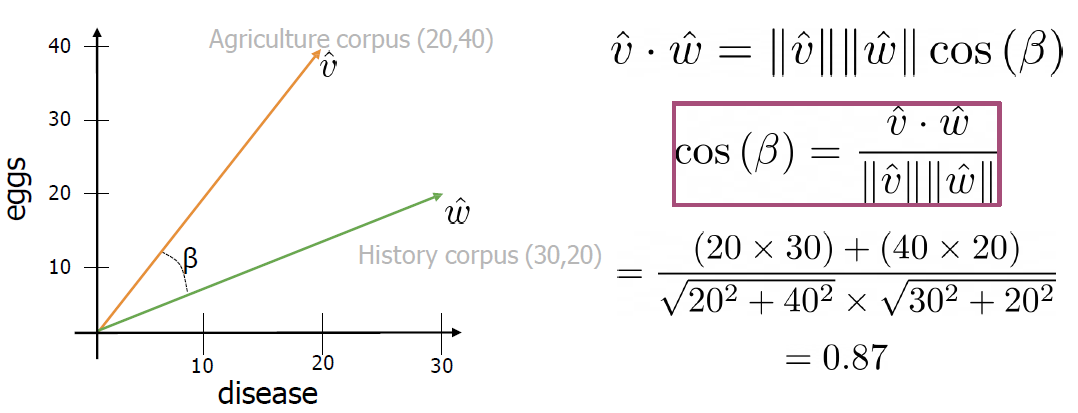
\includegraphics[width=\textwidth,height=0.65\textheight,keepaspectratio]{images/vector-space/cosine-similarity-1.png}
    \end{figure}
    \begin{itemize}
        \item Measures the cosine of the angle between two vectors.
        \item Formula: $\text{cosine}(\mathbf{x}, \mathbf{y}) = \frac{\mathbf{x} \cdot \mathbf{y}}{\|\mathbf{x}\| \|\mathbf{y}\|}$
        \item Ranges from -1 (opposite) to 1 (same direction).
        \item Less sensitive to magnitude, focuses on orientation.
    \end{itemize}
\framebreak
    \begin{figure}
        \centering
        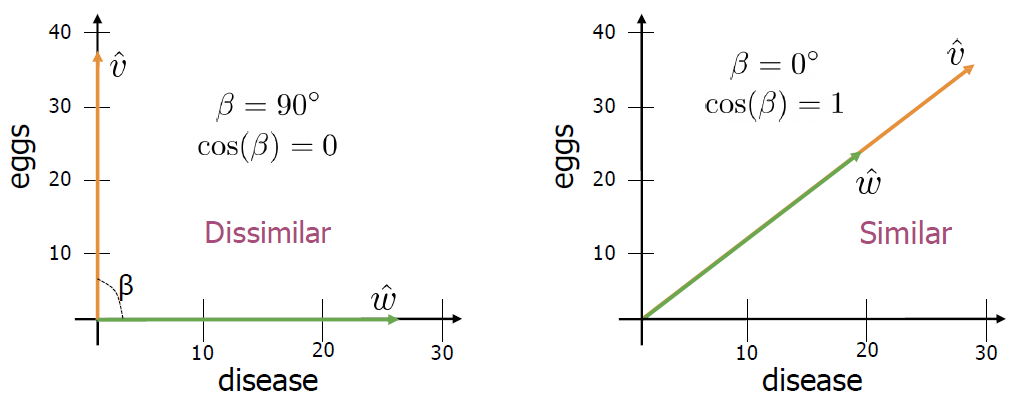
\includegraphics[width=\textwidth,height=0.8\textheight,keepaspectratio]{images/vector-space/cosine-similarity-2.png}
    \end{figure}
\end{frame}

\begin{frame}{Euclidean distance vs Cosine similarity}
    \begin{figure}
        \centering
        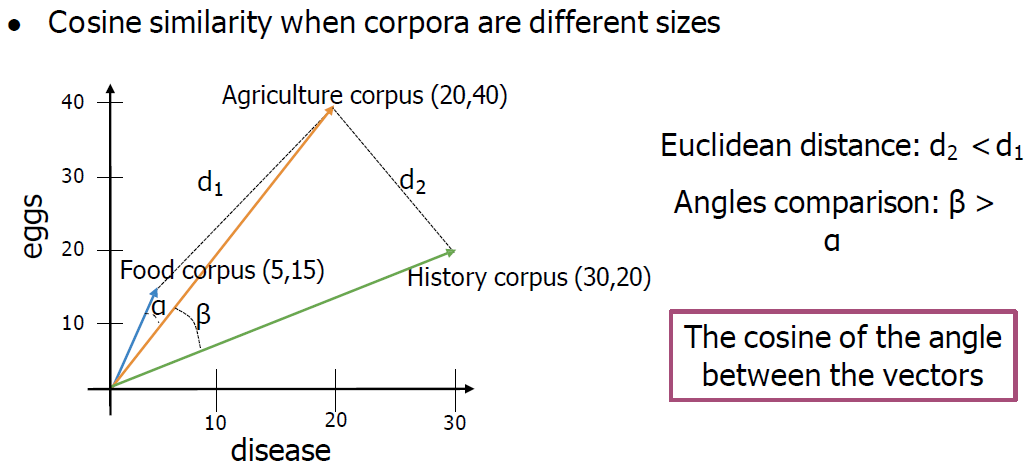
\includegraphics[width=\textwidth,height=0.8\textheight,keepaspectratio]{images/vector-space/euclidean-vs-cosine.png}
    \end{figure}
\end{frame}

\subsection{Manipulating word vectors}
\begin{frame}[allowframebreaks]{Manipulating word vectors}
    \begin{figure}
        \centering
        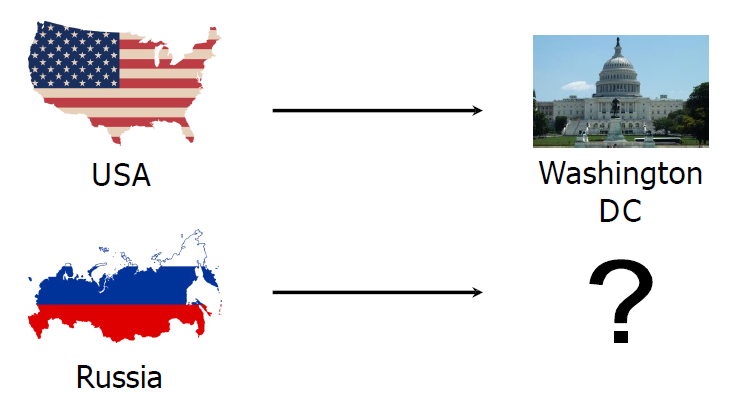
\includegraphics[width=\textwidth,height=0.65\textheight,keepaspectratio]{images/vector-space/manipulate-word-vec-1.png}
    \end{figure}
\framebreak
    \begin{figure}
        \centering
        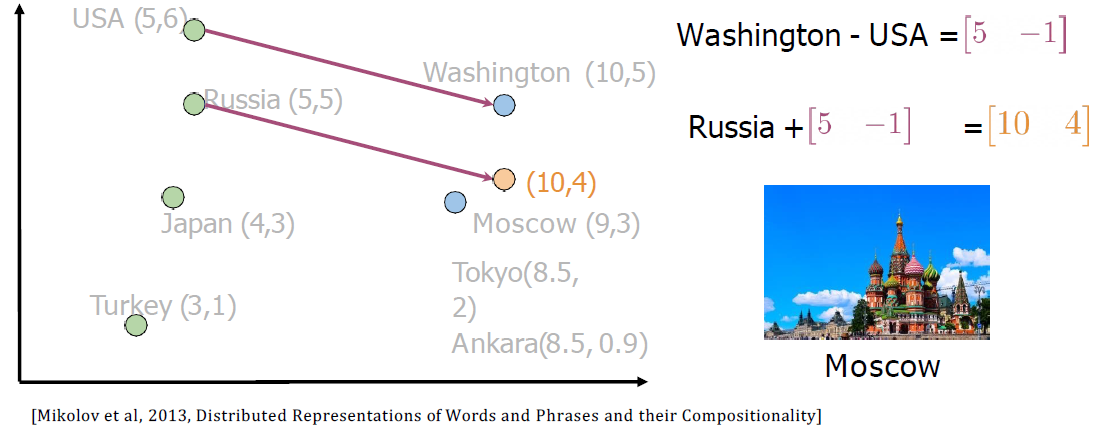
\includegraphics[width=\textwidth,height=0.8\textheight,keepaspectratio]{images/vector-space/manipulate-word-vec-2.png}
    \end{figure}
\end{frame}

\begin{frame}[allowframebreaks]{Visualization of word vectors}
    \foreach \i in {1,...,3} { % Integers from 1 to 5
        \begin{figure}
            \centering
            \includegraphics[height=0.8\textheight,width=1\textwidth,keepaspectratio]{images/vector-space/word-vec-vis-\i.png}
        \end{figure}

        \framebreak
    }
\end{frame}